\usetikzlibrary{positioning}

\begin{center}
    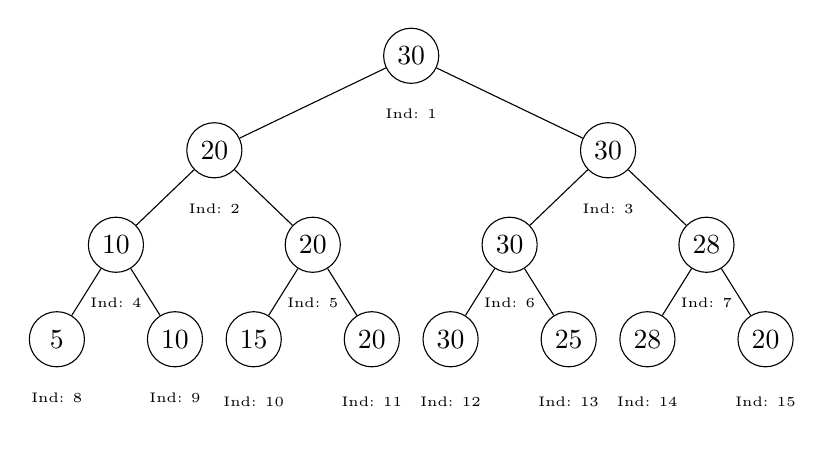
\begin{tikzpicture}[
      level distance=1.2cm,
      level 1/.style={sibling distance=5cm},
      level 2/.style={sibling distance=2.5cm},
      level 3/.style={sibling distance=1.5cm},
      every node/.style={draw,circle,minimum size=7mm,inner sep=1pt}
    ]
    
    % Tree nodes
    \node (n1) {30}
        child {node (n2) {20}
            child {node (n4) {10}
                child {node (n8) {5}}
                child {node (n9) {10}}
            }
            child {node (n5) {20}
                child {node (n10) {15}}
                child {node (n11) {20}}
            }
        }
        child {node (n3) {30}
            child {node (n6) {30}
                child {node (n12) {30}}
                child {node (n13) {25}}
            }
            child {node (n7) {28}
                child {node (n14) {28}}
                child {node (n15) {20}}
            }
        };
    
    % Small, tight Ind: labels
    \node[below=0.1pt of n1, draw=none, font=\tiny] {Ind: 1};
    \node[below=0.1pt of n2, draw=none, font=\tiny] {Ind: 2};
    \node[below=0.1pt of n3, draw=none, font=\tiny] {Ind: 3};
    \node[below=0.1pt of n4, draw=none, font=\tiny] {Ind: 4};
    \node[below=0.1pt of n5, draw=none, font=\tiny] {Ind: 5};
    \node[below=0.1pt of n6, draw=none, font=\tiny] {Ind: 6};
    \node[below=0.1pt of n7, draw=none, font=\tiny] {Ind: 7};
    \node[below=0.1pt of n8, draw=none, font=\tiny] {Ind: 8};
    \node[below=0.1pt of n9, draw=none, font=\tiny] {Ind: 9};
    \node[below=0.1pt of n10, draw=none, font=\tiny] {Ind: 10};
    \node[below=0.1pt of n11, draw=none, font=\tiny] {Ind: 11};
    \node[below=0.1pt of n12, draw=none, font=\tiny] {Ind: 12};
    \node[below=0.1pt of n13, draw=none, font=\tiny] {Ind: 13};
    \node[below=0.1pt of n14, draw=none, font=\tiny] {Ind: 14};
    \node[below=0.1pt of n15, draw=none, font=\tiny] {Ind: 15};
    
    \end{tikzpicture}
    \end{center}
    